%%%%%%%%%%%%%%%%%%%%%%%%%%%%%%%%%%%%%%%%%
%
% CMPT 435
% Spring 2019
% Lab One
%
%%%%%%%%%%%%%%%%%%%%%%%%%%%%%%%%%%%%%%%%%

%%%%%%%%%%%%%%%%%%%%%%%%%%%%%%%%%%%%%%%%%
% Short Sectioned Assignment
% LaTeX Template
% Version 1.0 (5/5/12)
%
% This template has been downloaded from: http://www.LaTeXTemplates.com
% Original author: % Frits Wenneker (http://www.howtotex.com)
% License: CC BY-NC-SA 3.0 (http://creativecommons.org/licenses/by-nc-sa/3.0/)
% Modified by Alan G. Labouseur  - alan@labouseur.com
%
%%%%%%%%%%%%%%%%%%%%%%%%%%%%%%%%%%%%%%%%%

%----------------------------------------------------------------------------------------
%	PACKAGES AND OTHER DOCUMENT CONFIGURATIONS
%----------------------------------------------------------------------------------------

\documentclass[letterpaper, 10pt]{article} 


\usepackage[english]{babel} % English language/hyphenation
\usepackage[utf8]{inputenc}
\usepackage{graphicx}
\usepackage[lined,linesnumbered,commentsnumbered]{algorithm2e}
\usepackage{listings}
\usepackage{minted}
\usepackage{fancyhdr} % Custom headers and footers
\pagestyle{fancyplain} % Makes all pages in the document conform to the custom headers and footers
\usepackage[table]{xcolor}
\usepackage{csquotes}
\usepackage{natbib}
\usepackage[nottoc]{tocbibind}
\usepackage{lastpage}
\usepackage{url}
\usepackage{float}
\usepackage{scrextend}
\usepackage{epigraph}
\fancyhead{} % No page header - if you want one, create it in the same way as the footers below
\fancyfoot[L]{} % Empty left footer
\fancyfoot[C]{page \thepage\ of \pageref{LastPage}} % Page numbering for center footer
\fancyfoot[R]{}
\usepackage{listings}% http://ctan.org/pkg/listings
\usepackage{hyperref}
\renewcommand{\headrulewidth}{0pt} % Remove header underlines
\renewcommand{\footrulewidth}{0pt} % Remove footer underlines
\setlength{\headheight}{13.6pt} % Customize the height of the header
\usepackage{pgfplots}

\pgfplotsset{width=7cm,compat=1.8}

%----------------------------------------------------------------------------------------
%	TITLE SECTION
%----------------------------------------------------------------------------------------

\newcommand{\horrule}[1]{\rule{\linewidth}{#1}} % Create horizontal rule command with 1 argument of height

\title{	
   \normalfont \normalsize 
   \textsc{CMPT 435 - Fall 2020 - Dr. Labouseur} \\[10pt] % Header stuff.
   \horrule{0.5pt} \\[0.25cm] 	% Top horizontal rule
   \large{Assignment Four -- Graphs and BSTs} \\
   \textsc{Graphs, Searching Graphs, Their Representations, and Binary Search Trees}\\[20pt]% Assignment title
 \author{Sam Alcosser \\ \normalsize Samuel.Alcosser1@Marist.edu}
   \horrule{0.5pt} \\ 	% Bottom horizontal rule
   


	% Today's date.
  
\date{\normalsize\today} 
}
\begin{document}




\fontfamily{bch}\selectfont
\maketitle
\tableofcontents
\newpage

\section{Introduction}

This document describes the implementations of Binary Search Trees and unweighted graphs, along with the methods associated with each. As seen in the table of contents, this document will follow the high level structure of first defining each of the data structure's implementations in detail, followed by an asymptotic running time analysis of the searching algorithms within each of the data structures.


\section{Binary Search Trees}
\begin{center}
    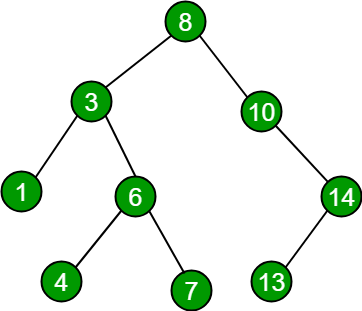
\includegraphics[width=\textwidth  / 2]{BST.png}

\end{center}

In a previous document, I described binary search as a way of strategically checking specific points in a set in order to close in on the desired value. Binary Search trees implement a similar strategy. With a binary Search tree, we connect our nodes in such a way that they usually have a parent node, and either, both, or neither a left and right node just as seen in the image above. The root node has no parent, we use this as the starting point for most of our operations. Below you see the header file for a node in a binary search tree I call \texttt{binNode.h}.

\begin{addmargin}[-5em]{1em}
\begin{small}
\begin{minted}[linenos=true]{cpp}
#pragma Once
#include <string>
class BinNode
{ 
public:
	std::string key; 
	BinNode* left = nullptr;		 
    BinNode* right = nullptr;
	BinNode* parent = nullptr;
};

\end{minted}
\end{small}
\end{addmargin}


As you can see, this is similar to the nodes seen in previous assignments, although now there are more pointers. One "pointing" to its parent, one down and to the left, and one down to the right. Just as seen in the graphic above, each node does not need to have both or even any child nodes, but all must have a parent node unless they are the root node.

\subsection{\texttt{BinTree.h}: Outline of Our Binary Search Tree Class}
 To begin, it is best to have a general understanding of some of the things that can be done with a binary search tree.
 
 \begin{addmargin}[-5em]{1em}
\begin{small}
\begin{minted}[linenos=true]{cpp}
#pragma once
#include <string>
#include <iostream>
#include "BinNode.h"

class BinTree{
    public:
    BinNode static search(BinNode * root, std::string key, int &count);
    void  insert(std::string key);
    BinNode * root;
    void pullBatch(std::string items[], int len);
};
\end{minted}
\end{small}
\end{addmargin}

\begin{itemize}
   \item \texttt{BinTree::search()} is the method we use to search our tree
   \item \texttt{BinTree::insert()} is used to insert a \texttt{BinNode} into the tree
   \item Our \texttt{root} pointer keeps tabs on where the start of the binary search tree is
   \item \texttt{BinTree::pullBatch()} is a function created to make large batch searches, such as the one in this assignment's case, much easier
   
\end{itemize}
\newpage
\subsection{\texttt{BinTree::insert()}: Inserting Into the BST}

The process of inserting a node into the tree is probably the most logically complex operation that will be done on the tree.


 \begin{addmargin}[-5em]{1em}
\begin{small}
\begin{minted}[linenos=true]{cpp}
void BinTree::insert(std::string key)
{
    BinNode *node = new BinNode();
    node->key = key;
    BinNode *ancestorNode = nullptr;
    BinNode *parent = root;
    while (parent != nullptr)
    {
        ancestorNode = parent;
        if (node->key < parent->key)
        {
            parent = parent->left;
        }
        else
        {
            parent = parent->right;
        }
    }
    node->parent = ancestorNode;
    if (ancestorNode == nullptr)
    {
        root = node;
    }
    else if (node->key < ancestorNode->key)
    {
        ancestorNode->left = node;
        //  std::cout  << "placed node left"<< std::endl;
    }
    else
    {
        ancestorNode->right = node;
        // std::cout  << "placed node right"<< std::endl;
    }
}
\end{minted}
\end{small}
\end{addmargin}

\begin{enumerate}
    \item First, a pointer to a new node is created with the string passed in by the \texttt{key} argument (lines 3,4).
    \item The trailing pointer \texttt{ancestorNode} and the parent pointer \texttt{parent} are initialized to \texttt{nullptr} and the root of the tree respectivley (lines 5,6).
    \item Within the while loop, \texttt{ancestorNode} stays one step behind \texttt{parent} (line 9) as they continue moving down left or right. This decision is made whether or not the new \texttt{binNode}'s \texttt{key} value is bigger or smaller than the parent's current position (left being smaller, right being bigger). This process continues until parent finds a \texttt{nullptr} on a node where the child can go.(lines 7-18).
    \item Now, the necessity to maintain a trailing \texttt{ancestorNode} is extremely apparent. Since it was constantly one step behind the \texttt{parent}, it just so happens that it is maintaining the pointer of the new node's parent pointer value which it is now assigned (line 19).
    \item If the \texttt{ancestorNode} is a \texttt{nullptr}, meaning that the tree is empty, assign the \texttt{root} pointer to the new node.(lines 20-23)
    \item  Otherwise, if the \texttt{node}'s \texttt{key} value is smaller than that of the \texttt{ancestorNode}, assign the new node to the \texttt{left} pointer of \texttt{ancestorNode}. Otherwise, assign it to the right. (lines 24-33)
\end{enumerate}

\subsection{\texttt{BinTree::search()}: Searching The Binary Search Tree}

As you may have realized, the way in which BSTs are set up makes them fairly easy to logically find values. The method I have implemented is a recursive way of searching for values within the tree.

 \begin{addmargin}[-5em]{1em}
\begin{small}
\begin{minted}[linenos=true]{cpp}
BinNode BinTree::search(BinNode *rNode, std::string key, int &count)
{
    if (rNode == nullptr || key == rNode->key)
    {
        count++;
        return *rNode;
    }
    else if (key < rNode->key)
    {
        count++;
        return search(rNode->left, key, count);
    }
    else
    {
        count++;
        return search(rNode->right, key, count);
    }
}
\end{minted}
\end{small}
\end{addmargin}

\begin{enumerate}
    \item In the rare case that the root node is a \texttt{nullptr}, or that the \texttt{key} passed into the function as an argument, return the root node from the function. This is derived by dereferencing the pointer to the parent node passed into the function initially.(lines 3-7)
    \item If the key is smaller than the key of the root node, continue the search starting at the left pointer of the current root node, using the same key.(lines 8-12)
    \item Otherwise, we can assume that the key is bigger, and therefore we will continue the search from the right pointer of the current parent node. (lines 13-17)
\end{enumerate}

\subsubsection{Asymptotic Running Time of \texttt{BinTree::search()}}
\textbf{Hold on,} how is the searching function the simplest operation for us? Well, If we start from the root node, we are simply looking if our key is bigger or smaller, then move down, wash, rinse, repeat. This is the elegance of the Binary Search Tree. When set up correctly, it can simplify the searching process greatly, as the process of inserting each element is effectivley sorting it as well. 

With this, the complexity of this search algorithm is only $O(log_2(n)$. The reason being that, just as with binary search in arrays, every time that we are comparing, we are effectively cutting our possible range in half. 

Although, one must be careful. If the order in which the binary search tree is filled is set in a particularly unlucky way, the complexity can climb up to $O(n)$. This can occur if the tree is filled in such a way that everything is just linked by the left pointer or only the right, effectively creating a linear search.

\subsection{\texttt{BinTree::pullBatch()}: A Streamlined Way For Batches Of Searches}

This function is relativley simple logically speaking, and therefore it doesn't require an in depth step by step analysis

 \begin{addmargin}[-5em]{1em}
\begin{small}
\begin{minted}[linenos=true]{cpp}
void BinTree::pullBatch(std::string items[], int len)
void BinTree::pullBatch(std::string items[], int len)
{

    int tCount = 0;
    for (int i = 0; i < len; i++)
    {
        int count = 0;
        auto res = search(root, items[i], count);
        std::cout << "Item "<< i+1 << " was found after " << count << " comparisons." << std::endl;
        tCount += count;
    }
    std::cout << "Total comparions to find all items: " << tCount << std::endl;
    int avg = tCount / len;
    std::cout << "Average comparisons to reach each item: " << avg << std::endl;
}
\end{minted}
\end{small}
\end{addmargin}

For every index in the array of items to find (line 6), search for it in the BST (line 9) and print and log the comparisons needed to find it (lines 10,11). Then when all of the items have been found, give the average comparisons by dividing the total comparisons by the number of items found(lines 13-15).


\section{Undirected Graphs}
\subsection{Introduction To Graphs}
 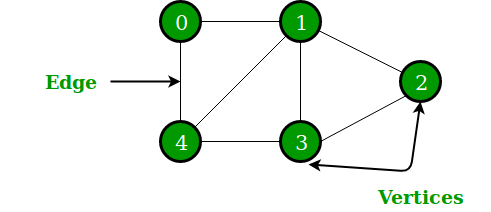
\includegraphics[width=\textwidth ]{undirectedgraph.png}
The data structure of an undirected graph is a set of vertices that can be connected to each other by edges. In order to represent the edges, each vertex on eah side of the edge reference eachother in their own array of neighbor vertices. In other words, if vertex $a$ and vertex $b$ share an edge, vertex $a$ would have a reference to vertex $b$, and vertex $b$ would have a reference to vertex $a$, both within their respective neighbors arrays.

\subsection{\texttt{Vertex.h}: The Smallest Unit Of A Graph}

As seen below, a single vertex is quite simple having only three parts.

 \begin{addmargin}[-5em]{1em}
\begin{small}
\begin{minted}[linenos=true]{cpp}
#pragma once
#include <iostream>
#include <vector>
class Vertex{
    public:
    int id;
    bool processed;
    std::vector<Vertex*> neighbors;
};
\end{minted}
\end{small}
\end{addmargin}
\begin{itemize}
    \item \texttt{id} holds the id of the vertex in an int
    \item \texttt{processed} is a sort of flag variable used when searching (more on this later)
    \item \texttt{std::vector<Vertex*> neighbors} is a used to hold a set of \texttt{Vertex} pointers as the neighbors of the vertex
\end{itemize}

\subsection{\texttt{GraphManager.h}: Maintaining The Graph}

The reason why I created a structure called \texttt{GraphManager} and not separate graph and searching and managing classes was simple. Since the vertices hold all of the necessary information within themselves, all there is to do to keep them together is to group them into a sort of list or array of some kind. Therefore, The whole class would only really be a vector. So, I instead decided to structure the whole set of operations within one class.

 \begin{addmargin}[-5em]{1em}
\begin{small}
\begin{minted}[linenos=true]{cpp}
#pragma once
#include <iostream>
#include <string>
#include <vector>
#include "Vertex.h"
class GraphManager{
    public:
    std::vector<Vertex*> graph;
    void Overlord(std::string fileName);
    void printAJList();
    void printMatrix();
    void BFSearch(Vertex* startV);
    void DFSearch(Vertex* startV);
    void resetVList();
    
};
\end{minted}
\end{small}
\end{addmargin}

\begin{itemize}
    \item \texttt{graph} holds a set of pointers to every vertex in the graph
    \item \texttt{Overlord()} is the function used to run all parts of the graph's functionality (this may seem like bad programming practice but I will explain later why this is done)
    \item \texttt{printAJList()} prints an adjacency list of the different vertices
    \item \texttt{printMatrix()} prints a matrix of the graph's vertices
    \item \texttt{BFSearch()} performs a breadth first search on the graph
    \item \texttt{DFSearch()} performs a depth first search on the graph
    \item \texttt{resetVList()} resets the \texttt{processed} flags on every vertex so that another search can be performed
\end{itemize}
\newpage
\subsection{Printing Methods}


These methods are used to show the data in the graphs in two different ways.

\subsubsection{\texttt{GraphManager::printAJList()}: Printing the Adjacency List}



\begin{addmargin}[-5em]{1em}
\begin{small}
\begin{minted}[linenos=true]{cpp}
void GraphManager::printAJList()
{
	std::cout << "---Printing Adjacency List---" << std::endl;
	for (int i = 0; i < graph.size(); i++)
	{
		std::cout << "[" << graph[i]->id << "]";
		for (int j = 0; j < graph[i]->neighbors.size(); j++)
		{
			std::cout << " " << graph[i]->neighbors[j]->id;
		}
		std::cout << std::endl;
	}
}
\end{minted}
\end{small}
\end{addmargin}

For each element in the graph as maintained by the \texttt{graph} vector, print out the id of that vertex and all of its neighbors next to it.




\newpage

\subsubsection{\texttt{GraphManager::printMatrix()}: Printing the Matrix}

\begin{addmargin}[-5em]{1em}
\begin{small}
\begin{minted}[linenos=true]{cpp}
void GraphManager::printMatrix()
{
	int size = graph.size();
	std::cout << "about to do matrix stuff" << std::endl;
	std::vector<std::vector<char>> matrix(size, std::vector<char>(size, '.'));
	std::cout << "--Printing Matrix--" << std::endl;

	//populating
	for (int i = 0; i < graph.size(); i++)
	{
		for (int j = 0; j < graph[i]->neighbors.size(); j++)
		{

			matrix[i][graph[i]->neighbors[j]->id] = '1';
		}
	}
	//printing
	std::cout << "    ";
	//table headings
	for (int n = 0; n < graph.size(); n++)
	{
		if (graph[n]->id < 10)
		{
			std::cout << graph[n]->id << "  ";
		}
		else
		{
			std::cout << graph[n]->id << " ";
		}
	}
	std::cout << std::endl;

	for (int i = 0; i < graph.size(); i++)
	{
		if (graph[i]->id < 10)
		{
			std::cout << " " << graph[i]->id << "| ";
		}
		else
		{
			std::cout << graph[i]->id << "| ";
		}
		//printing row by row

		for (int h = 0; h < matrix[i].size(); h++)
		{
			std::cout << matrix[i][h] << "  ";
		}
		std::cout << std::endl;
	}
}
\end{minted}
\end{small}
\end{addmargin}

\begin{enumerate}
    \item Initialize a 2D vector with a length and width equal to the number of vertices with periods to be used as a matrix. (lines 3,5)
    \item Use two nested for loops for populating. (lines 9-11).
    \item Use the outer loops iterator \texttt{i} and the inner loops \texttt{j} as vertex and neighbor indicators respectively. For every vertex \texttt{i}, place a 1 in the column of the neighbor at index \texttt{j}. (lines 9-16)
    \item print out each vertex's' id inline, leaving a single space if the id is 1 digit for consistency (lines 20-31)
    \item Start a for loop to iterate over each parent index in the matrix, as well as the index of the \texttt{graph} vector. (line 33)
    \item Start each line by giving a header of the id of the vertex at that index, leaving room again for single digit ids. (lines 35-42)
    \item For each character in the sub-vector of the current index, print out each value inline.(lines 45-49)
    
\end{enumerate}

\subsection{\texttt{Overlord()}: Running it all}

\texttt{Overlord()} is a function used to tie everything for the graphs together. Upon first glance, it may seem as if this function breaks a cardinal sin of programming by doing more than one thing in one function, although it is necessary. This function is more like a file reader, as its main purpose is to read in the text file and create a graph. Although, depending on the information on each line, it will add a vertex or edge, do nothing, or perform both print and searching processes on the graph. Then, the complexity of these functions are abstracted out into their own methods.

\begin{addmargin}[-5em]{1em}
\begin{small}
\begin{minted}[linenos=true]{cpp}
void GraphManager::Overlord(std::string fileName)
{

	std::fstream newfile;

	std::string ln;
	int count = 0;
	bool started = false;
	newfile.open(fileName, std::ios::in);
	if (newfile.is_open())
	{
		while (getline(newfile, ln)) //read each line of the file
		{

			if (ln.find("new graph") != std::string::npos)
			{

				if (started)
				{
					std::cout << "got to the printing" << std::endl;
					printAJList();
					printMatrix();
					BFSearch(graph[0]);
					resetVList();
					std::cout << "Printing elements as seen through Depth First Search" << std::endl;
					DFSearch(graph[0]);
					graph.clear();
				}
				started = true;
			}
			else if (ln.find("add vertex") != std::string::npos)
			{
				int id = std::stoi(ln.substr(11));
				Vertex *vertex = new Vertex();
				vertex->id = id;
				graph.push_back(vertex);
			}
			else if (ln.find("add edge") != std::string::npos)
			{

				int hyph = ln.find("-");

				int num1 = stoi(ln.substr((ln.find("edge") + 5), 2));
				int num2 = stoi(ln.substr(hyph + 2));

				for (int i = 0; i < graph.size(); i++)
				{
					if (graph[i]->id == num1)
					{
						for (int j = 0; j < graph.size(); j++)
						{
							if (graph[j]->id == num2)
							{
								graph[i]->neighbors.push_back(graph[j]);
								graph[j]->neighbors.push_back(graph[i]);
							}
						}
					}
				}
			}
		}
	}
	newfile.close();

	return;
};
\end{minted}
\end{small}
\end{addmargin}

\begin{enumerate}
    \item Begin processing the inputted file line by line. (line 1-12, 63)
    \item If the current line says "new graph" check if the graph has been started (line 15)
    \item If the graph has been started, meaning there is something in the graph, print the graph as an adjacency list, a matrix, then perform a breadth first and a depth first search while resetting the vertices processed flag in between the two.(lines 22-26)
    \item Clear the \texttt{graph} vector to begin a new graph.(line 27)
    \item If the line says "add vertex",  take the number on that line and make a vertex with that id. Then add it to the \texttt{graph} vector(lines 31-37)
    \item If the line says add edge, begin by parsing out both numbers. (lines 38-44)
    \item Using two nested for loops, find the vertex with the id of the first number (\texttt{i}) and then in an inner for loop locate the vertex with the id of the second number  (\texttt{j}).(lines 46-53)
    \item Add vertex with id \texttt{j} as a neighbor to vertex with id \texttt{i}, and vise versa.(lines 54,55)
    
\end{enumerate}












\subsection{\texttt{GraphManager::BFSearch}: Breadth First Search}

Breadth first search operates in a relatively simple fashion. As it progresses, it keeps iterating over each of the currently processing vertex's neighbors, seeing if those are processed, and if they are not, then putting them into a queue to be processed themselves.

\begin{addmargin}[-5em]{1em}
\begin{small}
\begin{minted}[linenos=true]{cpp}
void GraphManager::BFSearch(Vertex *startV)
{
	std::cout << "Printing elements as seen through Breadth First Search" << std::endl;
	Queue q = Queue();
	q.enQueue(startV);
	startV->processed = true;
	while (!q.isEmpty())
	{
		Vertex *cv = q.deQueue().data;
		std::cout << cv->id << std::endl;
		for (int i = 0; i < cv->neighbors.size(); i++)
		{
			if (!cv->neighbors[i]->processed)
			{
				q.enQueue(cv->neighbors[i]);
				cv->neighbors[i]->processed = true;
			}
		}
	}
	std::cout << "------------------------------" << std::endl;
}
\end{minted}
\end{small}
\end{addmargin}

\begin{enumerate}
    \item Begin a \texttt{Queue} and place the starting vertex \texttt{startV} on it.  (lines 4, 5)
    \item Mark the starting vertex as processed. (line 6)
    \item Open a while loop that will run until the queue is empty. (line 7)
    \item Set our current vertex \texttt{cv} to the value of the \texttt{data} field in the next \texttt{node} to be \texttt{deQueue}d from the queue.(line 9)
    \item Print the id of the \texttt{vertex}.(line 10)
    \item Begin a for loop that will iterate over each index in the vector of neighbors on the current vertex.(line 11)
    \item if the neighbor of the current vertex indicated by the currently operating index is not yet processed, add said neighbor to the queue and set it to processed. (lines 13-17)
\end{enumerate}
\subsubsection{Asymptotic Running Time Analysis Of \texttt{BFSearch()}}

By having a while loop and a for loop nested inside of it, upon first glance one may think that this process is relatively complex in terms of running time. Although there are two things to keep in mind. First of all, most of the operations in this function operate in constant time. Also, in reality we are not operating with a set of sets of data as it may seem, but instead we are operating with a simple list of elements that are all interconnected.

So, when the process is going through each vertex, each of its neighbors, and each of its neighbors and so on, it is all the same set of data. Because of this, breadth first search is actually $O(V+E)$, as the worst case would be that the algorithm has to go to every vertex and every edge. Therefore, this operation's runtime is linear.

\subsection{\texttt{GraphManager::DFSearch}: Depth First Search}

Depth first search is different from breadth first in a couple of ways. First of all, as the name implies, the algorithm processes the vertices by going depth first, trying to go through all of the neighbors of one vertex instead of jumping around as breadth first search does.

\begin{addmargin}[-5em]{1em}
\begin{small}
\begin{minted}[linenos=true]{cpp}
void GraphManager::DFSearch(Vertex *startV)
{

	if (!startV->processed)
	{
		std::cout << startV->id << std::endl;
		startV->processed = true;
	}
	for (int i = 0; i < startV->neighbors.size(); i++)
	{
		if (!startV->neighbors[i]->processed)
		{
			DFSearch(startV->neighbors[i]);
		}
	}
}

\end{minted}
\end{small}
\end{addmargin}

\begin{enumerate}
    \item If the starting vertex is not processed, print its' id and mark it as processed. (lines 4-8)
    \item Start a for loop that will be used to iterate over every neighbor of the starting vertex (line 9)
    \item If the neighbor in focus in this iteration is not processed, perform a depth first search starting at this neighbor. (lines 11-14)
\end{enumerate}

\subsubsection{Asymptotic Running Time Of \texttt{DFSearch}}

Just like breadth first search, depth first search is also a linear time operation. The only difference again being that breadth first focuses on getting a hold of each part of the graph, while depth first attempts to fully process each vertex as much as it can. Despite these differences, depth first still has to walk over or process each vertex and edge, giving it the same runtime of $O(V+E)$.

\section{\texttt{Main::main()}: Execution}

\texttt{Main::main()} is in all honestly a very simple funcion. And for good reason! By properly abstracting my code, I was able to build a main function that is simple and not messy, yet I still am well aware of what is being executed.
\begin{addmargin}[-5em]{1em}
\begin{small}
\begin{minted}[linenos=true]{cpp}
int main(){
	setupMagic();
    BinTree * tree = new BinTree();
    populateTree(tree, arr, MAGIC_LEN);
	string randItems[CHOSEN_LEN];
	randPick(arr, randItems, MAGIC_LEN, CHOSEN_LEN);
	tree->pullBatch(randItems, CHOSEN_LEN);
	GraphManager * gm = new GraphManager();
	gm->Overlord("graphs1.txt");
	return 0;
}
\end{minted}
\end{small}
\end{addmargin}

\begin{itemize}
    \item \texttt{setupMagic()} condenses all of the processes needed to initialize the array of 666 items into a single function. THis is not covered as the same code has been carried over with little to no alteration.
    \item \texttt{tree} becomes the tree we will use for our operations
    \texttt{populateTree()} goes through and calls the \texttt{BinTree::insert()} function on all of the items in the array of the magic items.
    \item Lines 5-7 create a list of 24 random items from the same array and search for them all using \texttt{pullBatch()}. This function simplifies the process at this point by making it easier to do all at once
    \item All that is left is to create a \texttt{GraphManager} and call \texttt{Overlord()} on it.(lines 8,9)
    
\end{itemize}






\section{Conclusion}
\subsection{Results}
\begin{center}
{\rowcolors{2}{gray!50}{white!100}
 \begin{tabular}{||c c c c||} 
 \hline
 Search Algorithm & Complexity/ $O()$\\ [0.5ex] 
 \hline\hline
  Breadth First Search & $O(V+E)$\\
   \hline
 Depth First Search & $O(V+E)$\\ 
 \hline
 Binary Tree Search&$O(log_2(n))$\\



 \hline
\end{tabular}
}
\end{center}

Here I have put all of the searching algorithms in one place so it is easier to compare.

\subsection{References}

Cormen, Thomas H., et al. Introduction to Algorithms. MIT Press, 2007.

\vspace{1.5em}

Geeks, Geeks For. “Check If given Sorted Sub-Sequence Exists in Binary Search Tree.” GeeksforGeeks, 21 May 2019, www.geeksforgeeks.org/check-if-given-sorted-sub-sequence-exists-in-binary-search-tree/.

\vspace{1.5em}

Geek. “Graph Data Structure And Algorithms.” GeeksforGeeks, www.geeksforgeeks.org/graph-data-structure-and-algorithms/.

\newpage


\textbf{Closing Thoughts: A Story}

The week prior to handing this in, I was having major troubles with my \texttt{Overlord()} function when I was trying to add edges. I just assumed it was an issue with pointers, as clearly that is usually my issue. I left it alone for a day, as I was stumped and could not find the answer. I even opened an online compiler to try and replicate my problem, but it worked! So I had completely lost hope. Then that night a friend from home who is trying to get into computer science texted me. 

He wanted my help understanding how for loops work. I felt so high and mighty giving him an in depth explanation of how they work, being happy that I can be of help to him. Then the next day I returned to the same code and got mad at the screen for another hour or so. But then, I realized my mistake. A for loop inside of the function that should look like \newline \texttt{for (int j = 0; j < graph.size(); j++)} actually read \newline \texttt{for (int j = 0;graph.size(); j++)}. I doubt I'll ever make that mistake again.
\newline

as a wise person once said, "
give a person a program and they'll be
frustrated for a day, teach a person to
program and they'll be frustrated for the
rest of their life.".
 \vspace{.5em}
{\textit{\color{red}\huge{\{S.A.\}}}}
\vspace{1em}
\end{document}

